\documentclass[a4paper]{article}

\usepackage[a4paper,margin=1in]{geometry}
\usepackage{graphicx}

\usepackage[utf8]{inputenc}
\usepackage[T1]{fontenc}
%\usepackage{amsthm}
\usepackage{tikz}

\setlength{\parindent}{0cm}
\setlength{\parskip}{1ex}
\setlength{\itemsep}{3ex}

\setlength{\fboxsep}{0pt}

%\theoremstyle{definition}
\newtheorem{definition}{Definition}

\begin{document}

\tableofcontents

\newpage
\section{Introduction}
Given is a tabular dataset $T$.
Observation tells us that sometimes one can predict some (im-)possible values in one column if the value of an other column is given.

Best example is the \texttt{user-id} and the \texttt{student-id} in a list of all marks for homework in a semester.
Both values usually appear many times but every \texttt{student-id} is matches exactly to one \texttt{user-id}.
We could give a function $f : \texttt{student-id} \to \texttt{user-id}$.
So the \texttt{user-id} is functional dependent to the \texttt{student-id}.
In this example you can we have a special case called bijection as the \texttt{student-id} is functional dependent to the \texttt{user-id} too.
In this case we can easy remove one of these columns and use the function to create the value of this column for a row if needed.

An other example would be the columns \texttt{patient-id} and \texttt{gender} in a table of clinical measurements. 
Value in the column \texttt{patient-id} may or may not repeated.
Usually the gender don't change and we have a function $f : \texttt{patient-id} \to \{ \mbox{female}, \mbox{male} \}$.
As there are usually more than two patients it is obvious that there is no function that maps from \texttt{gender} into \texttt{patient-id}. 

To check if two columns are functional dependent we can do as follow:
\begin{itemize}
\item Build the sets of all used values.\\ (e.g: $A = \{ x : x \mbox{ is in the first column} \}$ and $B = \{ x : x \mbox{ is in the second column} \}$)
\item Consider the relation $\sim_T$ between $A$ and $B$ given by the tables. With $a \sim_T b \Leftrightarrow a$ and $b$ are in the same row in the table for $a \in A$ and $b \in B$.
\item $B$ is functional dependent by $A$ iff for every $a \in A$ there is exactly one $b \in B$.
\end{itemize}

But what is if there is no mapping possible but we know that there are some limitations in $B$ for some values in $A$.
For example that for a table $A = \{ \mbox{female}, \mbox{male} \}$ and $B = \{ \mbox{pregnant}, \mbox{not-pregnant} \}$.
In this case we might have female $\sim_T$ pregnant, female $\sim_T$ not-pregnant and male $\sim_T$ not-pregnant but never \mbox{male $\sim_T$ pregnant}.
Such a case is logically dependency.
We would get a function $F$ that maps $A$ to the powerset of $B$ by $F(a) = \{ b \in B : a \sim_T b \}$. 
In this case $F(\mbox{female}) \{ \mbox{pregnant}, \mbox{not-pregnant} \}$ and $F(\mbox{male}) \{ \mbox{not-pregnant} \}$.

Using this we can say:
\begin{itemize}
\item $B$ is logical dependent by $A$ in table $T$ iff $|F(a)| < |B|$ for at least one $a \in A$.
\item $B$ is functional dependent by $A$ in table $T$ iff $|F(a)| = 1$ for all $a \in A$.
\item There is a bijection between $A$ and $B$ iff $B$ is functional dependent by $A$ and $A$ is functional dependent by $B$.
\end{itemize}

An open question is: can we find a function $Q$ that takes two columns of a table and give us a number that gives us a feeling how good the logical dependency between this two columns is?



\section{Definitions}

\begin{enumerate}
\item The set $[m \ldots n] = \{ m, m + 1, m + 2, \ldots, n \}$ for $m \leq n$.

\item $\mathcal{P}(M)$ denotes the powerset of the set $M$. So $\mathcal{P}(M) = \{ S : S \subseteq M \}$

\item $T$ in a table with $M \geq 2$ columns and $N \geq 1$ rows.

\item Consider two different columns in $T$.
      Let this be $(a_i)_{i \in [1 \ldots N]}$ and $(b_i)_{i \in [1 \ldots N]}$.

\item Let $A$ and $B$ the sets of the present values in this columns.
      \\ $A = \{ a_i : i \in [1 \ldots N] \}$ and $B = \{ b_i : i \in [1 \ldots N] \}$.

\item The table $T$ produces a relation $\sim_T$ between $A$ and $B$ by $a \sim_T b$ if and only if there is a row in $T$ where $a \in A$ and $b \in B$ are in the same row.
      With other words: 
      \[
          \mbox{for all } a \in A, b \in B \mbox{ it holds that }  a \sim_T b \Leftrightarrow \mbox{ there is an } i \in [1..N] \mbox{ with }a_i = a \mbox{ and } b_i = b
      \]

\item The function $F ; A \to \mathcal{P}(B)$ defined as $F(a) = \{ b \in B : a \sim_T b \}$ gives us all possible $b \in B$ for a given $a \in A$.

%\item Let $P(a,b)$ be the conditional probability that we find a row with $(a,b)$ is in $T$ for a given $a$. E.g:
%\[
%  P(a,b) = \frac{| \{ i \in [1 \ldots N] : a_i = a \mbox{ and } b_i = b\} |}{| \{ i \in [1 \ldots N] : a_i = a \} |}
%\]
\end{enumerate}

\section{The function $Q_T$}

The wishlist:
\begin{itemize}
\item $Q_T(A,B)$ should be zero if $T$ produces a function $f : A \to B$
\item $Q_T(A,B)$ should be one if for every $a \in A$ and $b \in B$ the relation $a \sim_T b$ holds.
\item Every other value of $Q_T(A,B)$ should be between zero and one
\end{itemize}


For a given $a \in A$ we can count how many $b \in B$ holds $a \sim_T b$ by $n = |F(a)| = |\{ b \in B : a \sim_T b \}|$
The more values are excluded the closer we are to a function that takes this $a$ and gives us a $b$.
If there is a function from $A$ to $B$ for this value $a$ then $n = 1$.
By the definition of our Table (not empty) and $A, B$ (= sets of the actual values in the table) we know that $n$ has to be greater or equal to 1.
By subtracting 1 we get: $n' = |F(a)| - 1 \geq 0$

If $a \sim_T b$ for all $b\in B$ for this $a \in A$ then $n' = |B| - 1$.
Assuming $|B| > 1$ we can divide this value and get the function:
\[
  Q_B(a) = \frac{|F(a)| - 1}{|B| - 1}
\]
that maps to the interval $[0, 1]$.
We can sum this up by 
\[
  s = \sum_{a \in A} Q_B(a)
  = \sum_{a \in A} \frac{|F(a)| - 1}{|B| - 1}
  = \frac{1}{|B| - 1} \sum_{a \in A} (|F(a)| - 1)
\]

We can easily see that $s \in [0, |A|]$.

Dividing $|A|$ gives us one solution to our wishlist for $|B| > 1$:
\[
  s' = \frac{s}{|A|}
  = \frac{1}{|A| \cdot (|B| - 1)} \sum_{a \in A} (|F(a)| - 1)
  = \frac{1}{|A| \cdot (|B| - 1)} \sum_{a \in A} (|\{ b \in B : a \sim_T b \}| - 1)
\]
If we put $a$ in the set we can omit the sum and get the easier term:
\[
  s' = \frac{|\{ (a,b) : a \in A, b \in B \mbox{ and } a \sim_T b \}| - |A|}{|A| \cdot (|B| - 1)}
\]

For the special case that there is only one value in column $B$ (e.g: $B = \{ b \}$) we have the obvious constant function $f(a) = b$.
This leads to our final definition:

\begin{equation}
\begin{array}{lll}
 Q_T( A, B ) & = \frac{|\{ (a,b) : a \in A, b \in B \mbox{ and } a \sim_T b \}| - |A|}{|A| \cdot (|B| - 1)} & ; if |B| > 1 \\
 Q_T(A, B)   & = 0  & ; if |B| \leq 1 
\end{array}
\end{equation}


\newpage
\section{Comparing two Tables}

Let $T$ and $T'$ be tables with columns \texttt{A} and \texttt{B}.
$T'$ might be a synthetic generated dataset from the real dataset $T$.
So the content in the columns might differ between the tables.

Let $F_{\tau, M}(a) = \{ x \in M : a \sim_\tau x \}$

\begin{equation}
  \Delta_{T,T'}(A, B) = \frac{1}{|A|} 
    \sum_{a \in A}
    \frac{\left|F_{T, B}(a) \cap F_{T', B}(a)\right|}{|F_{T, B}(a)|}
    \cdot
    \frac{\left|\left(B \setminus F_{T, B}(a)\right) \cap \left(B \setminus F_{T', B}(a)\right)\right|}{|B \setminus F_{T, B}(a)|}
\end{equation}





\newpage
\section{Additionally thoughts}
\subsection{More than one column as source or destination}
Assume we have a table with the columns \texttt{X}, \texttt{Y} and \texttt{B}.
Assume we want to check if the table gives us a function $f(x,y) = b$.
%Again let be
%  $B = \{ b : b \mbox{ is in column \texttt{B}} \}$,
%  $X = \{ x : x \mbox{ is in column \texttt{X}} \}$ and 
%  $Y = \{ y : y \mbox{ is in column \texttt{Y}} \}$.
  Create a new column \texttt{A} with $a_i = (x_i, y_i)$ for all rows $i \in [1 \ldots N]$. 
  Using this new column we can use $Q_T(A,B)$ to test the quality of logical dependency between $A \subseteq X \times Y$ and $B$. 

\subsection{Bipatite Graphs}
The relation $\sim_T$ builds a bipartite graph.
With $A$ as nodes on one side, $B$ as nodes on the other side and edges when $a \sim_T b$.

We can add a weight to the edges by the conditional probability $P(b|a)$.
Question: Is it possible that this gives some additional insights?


\subsection{Open questions}
\begin{itemize}
\item how to interpret the non obvious values $> 0$ and $< 1$?
\item how to compare two tables (e.g. real and synthetic data)?
\item What additional information about a table we can produce with this?
\end{itemize}



\subsection{Interprations of $Q_T(A,B)$}
Concider $n_a = |A| \times Q_T(A,B)$. 

\begin{definition}[Signature $S_{T,B}(A)$]
  Let $s_{T,B}(a) = |\{ b \in B : a \sim_T b \}|$.

  Let $(a_i)_{i \in [1 \ldots |A|]} \in A$ with $a_i \neq a_j$ for $i \neq j$.
  So $A = \{ a_i : i \in [1 \ldots |A|] \}$.

  Let $a_i$ is sorted in such way that $a_i \leq a_j$ for $i < j$.

  Define the signature $S_{T,B}(A)$ of $~_T$ for column $A$ to column $B$ as the following vector:
  \begin{equation}
    S_{T,B}(A) = (s_{T,B}(a_1), s_{T,B}(a_2), s_{T,B}(a_3), \ldots )
  \end{equation}
\end{definition}

The signature gives us a hint how the relation is distributed.
The sorting helps to normalize the signature and leads to lesser cases to consider as you could simply rename the items in the sets to get a equivalent relation with different sorting.

\begin{tabular}{c|c|l}
$Q_T(A,B)$ & $|A| \times Q_T(A,B)$ & signature $S_{T,B}(A)$ \\\hline
 0.000 & 0.000 & 1111 \\
 0.083 & 0.333 & 1112 \\
 0.167 & 0.667 & 1113 1122 \\
 0.250 & 1.000 & 1114 1123 1222 \\
 0.333 & 1.333 & 1124 1133 1223 2222 \\
 0.417 & 1.667 & 1134 1224 1233 2223 \\
 0.500 & 2.000 & 1144 1234 1333 2224 2233 \\
 0.583 & 2.333 & 1244 1334 2234 2333 \\
 0.667 & 2.667 & 1344 2244 2334 3333 \\
 0.750 & 3.000 & 1444 2344 3334 \\
 0.833 & 3.333 & 2444 3344 \\
 0.917 & 3.667 & 3444 \\
 1.000 & 4.000 & 4444
\end{tabular}
% \hfill
% \begin{tikzpicture}
% %Nodes
% \node  (nodeTitle) at (3,3.5) {Example for 1144};
% \node  (nodeA) at (0,3) {Alice};
% \node  (nodeB) at (0,2) {Bob};
% \node  (nodeC) at (0,1) {Charlie};
% \node  (nodeD) at (0,0) {Dave};
% \node  (nodeChocolate) at (6,3) {Chocolate};
% \node  (nodeVanilla)   at (6,2) {Vanilla};
% \node  (nodeBlueberry) at (6,1) {Blueberry};
% \node  (nodeRaspberry) at (6,0) {Raspberry};
% 
% %Lines
% \draw[->] (nodeA) edge node[thick, auto] {} (nodeChocolate);
% 
% \draw[->] (nodeB) edge node[thick, auto] {} (nodeVanilla);
% 
% \draw[->] (nodeC) edge node[thick, auto] {} (nodeRaspberry);
% \draw[->] (nodeC) edge node[thick, auto] {} (nodeBlueberry);
% \draw[->] (nodeC) edge node[thick, auto] {} (nodeChocolate);
% \draw[->] (nodeC) edge node[thick, auto] {} (nodeVanilla);
% 
% \draw[->] (nodeD) edge node[thick, auto] {} (nodeChocolate);
% \draw[->] (nodeD) edge node[thick, auto] {} (nodeVanilla);
% \draw[->] (nodeD) edge node[thick, auto] {} (nodeBlueberry);
% \draw[->] (nodeD) edge node[thick, auto] {} (nodeRaspberry);
% \end{tikzpicture}
% 
% ~
% 
% \begin{tikzpicture}
% %Nodes
% \node  (nodeTitle) at (3,3.5) {Example for 1234};
% \node  (nodeA) at (0,3) {Alice};
% \node  (nodeB) at (0,2) {Bob};
% \node  (nodeC) at (0,1) {Charlie};
% \node  (nodeD) at (0,0) {Dave};
% \node  (nodeChocolate) at (6,3) {Chocolate};
% \node  (nodeVanilla)   at (6,2) {Vanilla};
% \node  (nodeBlueberry) at (6,1) {Blueberry};
% \node  (nodeRaspberry) at (6,0) {Raspberry};
% 
% %Lines
% \draw[->] (nodeA) edge node[thick, auto] {} (nodeChocolate);
% 
% \draw[->] (nodeB) edge node[thick, auto] {} (nodeVanilla);
% \draw[->] (nodeB) edge node[thick, auto] {} (nodeChocolate);
% 
% \draw[->] (nodeC) edge node[thick, auto] {} (nodeRaspberry);
% \draw[->] (nodeC) edge node[thick, auto] {} (nodeBlueberry);
% \draw[->] (nodeC) edge node[thick, auto] {} (nodeVanilla);
% 
% \draw[->] (nodeD) edge node[thick, auto] {} (nodeChocolate);
% \draw[->] (nodeD) edge node[thick, auto] {} (nodeVanilla);
% \draw[->] (nodeD) edge node[thick, auto] {} (nodeBlueberry);
% \draw[->] (nodeD) edge node[thick, auto] {} (nodeRaspberry);
% \end{tikzpicture}
% \hfill
% \begin{tikzpicture}
% %Nodes
% \node  (nodeTitle) at (3,3.5) {Example for 1333};
% \node  (nodeA) at (0,3) {Alice};
% \node  (nodeB) at (0,2) {Bob};
% \node  (nodeC) at (0,1) {Charlie};
% \node  (nodeD) at (0,0) {Dave};
% \node  (nodeChocolate) at (6,3) {Chocolate};
% \node  (nodeVanilla)   at (6,2) {Vanilla};
% \node  (nodeBlueberry) at (6,1) {Blueberry};
% \node  (nodeRaspberry) at (6,0) {Raspberry};
% 
% %Lines
% \draw[->] (nodeA) edge node[thick, auto] {} (nodeChocolate);
% 
% \draw[->] (nodeB) edge node[thick, auto] {} (nodeVanilla);
% \draw[->] (nodeB) edge node[thick, auto] {} (nodeChocolate);
% \draw[->] (nodeB) edge node[thick, auto] {} (nodeBlueberry);
% 
% \draw[->] (nodeC) edge node[thick, auto] {} (nodeRaspberry);
% \draw[->] (nodeC) edge node[thick, auto] {} (nodeBlueberry);
% \draw[->] (nodeC) edge node[thick, auto] {} (nodeVanilla);
% 
% \draw[->] (nodeD) edge node[thick, auto] {} (nodeVanilla);
% \draw[->] (nodeD) edge node[thick, auto] {} (nodeBlueberry);
% \draw[->] (nodeD) edge node[thick, auto] {} (nodeRaspberry);
% \end{tikzpicture}
% 
% ~
% 
% \begin{tikzpicture}
% %Nodes
% \node  (nodeTitle) at (3,3.5) {Example for 2224};
% \node  (nodeA) at (0,3) {Alice};
% \node  (nodeB) at (0,2) {Bob};
% \node  (nodeC) at (0,1) {Charlie};
% \node  (nodeD) at (0,0) {Dave};
% \node  (nodeChocolate) at (6,3) {Chocolate};
% \node  (nodeVanilla)   at (6,2) {Vanilla};
% \node  (nodeBlueberry) at (6,1) {Blueberry};
% \node  (nodeRaspberry) at (6,0) {Raspberry};
% 
% %Lines
% \draw[->] (nodeA) edge node[thick, auto] {} (nodeChocolate);
% \draw[->] (nodeA) edge node[thick, auto] {} (nodeVanilla);
% 
% \draw[->] (nodeB) edge node[thick, auto] {} (nodeVanilla);
% \draw[->] (nodeB) edge node[thick, auto] {} (nodeChocolate);
% 
% \draw[->] (nodeC) edge node[thick, auto] {} (nodeRaspberry);
% \draw[->] (nodeC) edge node[thick, auto] {} (nodeBlueberry);
% 
% \draw[->] (nodeD) edge node[thick, auto] {} (nodeChocolate);
% \draw[->] (nodeD) edge node[thick, auto] {} (nodeVanilla);
% \draw[->] (nodeD) edge node[thick, auto] {} (nodeBlueberry);
% \draw[->] (nodeD) edge node[thick, auto] {} (nodeRaspberry);
% \end{tikzpicture}
% \hfill
% \begin{tikzpicture}
% %Nodes
% \node  (nodeTitle) at (3,3.5) {Example for 2233};
% \node  (nodeA) at (0,3) {Alice};
% \node  (nodeB) at (0,2) {Bob};
% \node  (nodeC) at (0,1) {Charlie};
% \node  (nodeD) at (0,0) {Dave};
% \node  (nodeChocolate) at (6,3) {Chocolate};
% \node  (nodeVanilla)   at (6,2) {Vanilla};
% \node  (nodeBlueberry) at (6,1) {Blueberry};
% \node  (nodeRaspberry) at (6,0) {Raspberry};
% 
% %Lines
% \draw[->] (nodeA) edge node[thick, auto] {} (nodeChocolate);
% \draw[->] (nodeA) edge node[thick, auto] {} (nodeVanilla);
% 
% \draw[->] (nodeB) edge node[thick, auto] {} (nodeVanilla);
% \draw[->] (nodeB) edge node[thick, auto] {} (nodeChocolate);
% 
% \draw[->] (nodeC) edge node[thick, auto] {} (nodeRaspberry);
% \draw[->] (nodeC) edge node[thick, auto] {} (nodeBlueberry);
% \draw[->] (nodeC) edge node[thick, auto] {} (nodeVanilla);
% 
% \draw[->] (nodeD) edge node[thick, auto] {} (nodeVanilla);
% \draw[->] (nodeD) edge node[thick, auto] {} (nodeBlueberry);
% \draw[->] (nodeD) edge node[thick, auto] {} (nodeRaspberry);
% \end{tikzpicture}

~

% Same examples as tables:\\
\begin{tabular}{c||c|c|c|c}
1144 & $B_1$ & $B_2$ & $B_3$ & $B_4$ \\\hline\hline
 $A_1$ & x & ~ & ~ & ~ \\
 $A_2$ & x & ~ & ~ & ~ \\
 $A_3$ & x & x & x & x \\
 $A_4$ & x & x & x & x \\
\end{tabular}
\hfill
\begin{tabular}{c||c|c|c|c}
1234 & $B_1$ & $B_2$ & $B_3$ & $B_4$ \\\hline\hline
 $A_1$ & x & ~ & ~ & ~ \\
 $A_2$ & x & x & ~ & ~ \\
 $A_3$ & x & x & x & ~ \\
 $A_4$ & x & x & x & x \\
\end{tabular}
\hfill
\begin{tabular}{c||c|c|c|c}
1333 & $B_1$ & $B_2$ & $B_3$ & $B_4$ \\\hline\hline
 $A_1$ & x & ~ & ~ & ~ \\
 $A_2$ & x & x & x & ~ \\
 $A_3$ & x & x & x & ~ \\
 $A_4$ & x & x & x & ~ \\
\end{tabular}

\begin{tabular}{c||c|c|c|c}
2224 & $B_1$ & $B_2$ & $B_3$ & $B_4$ \\\hline\hline
 $A_1$ & x & x & ~ & ~ \\
 $A_2$ & x & x & ~ & ~ \\
 $A_3$ & x & x & ~ & ~ \\
 $A_4$ & x & x & x & x \\
\end{tabular}
\hfill
\begin{tabular}{c||c|c|c|c}
2233 & $B_1$ & $B_2$ & $B_3$ & $B_4$ \\\hline\hline
 $A_1$ & x & x & ~ & ~ \\
 $A_2$ & x & x & ~ & ~ \\
 $A_3$ & x & x & x & ~ \\
 $A_4$ & x & x & x & ~ \\
\end{tabular}


~


\begin{minipage}{\textwidth}
By adding only one relation you can traverse through the possible relations like following:

\begin{center}
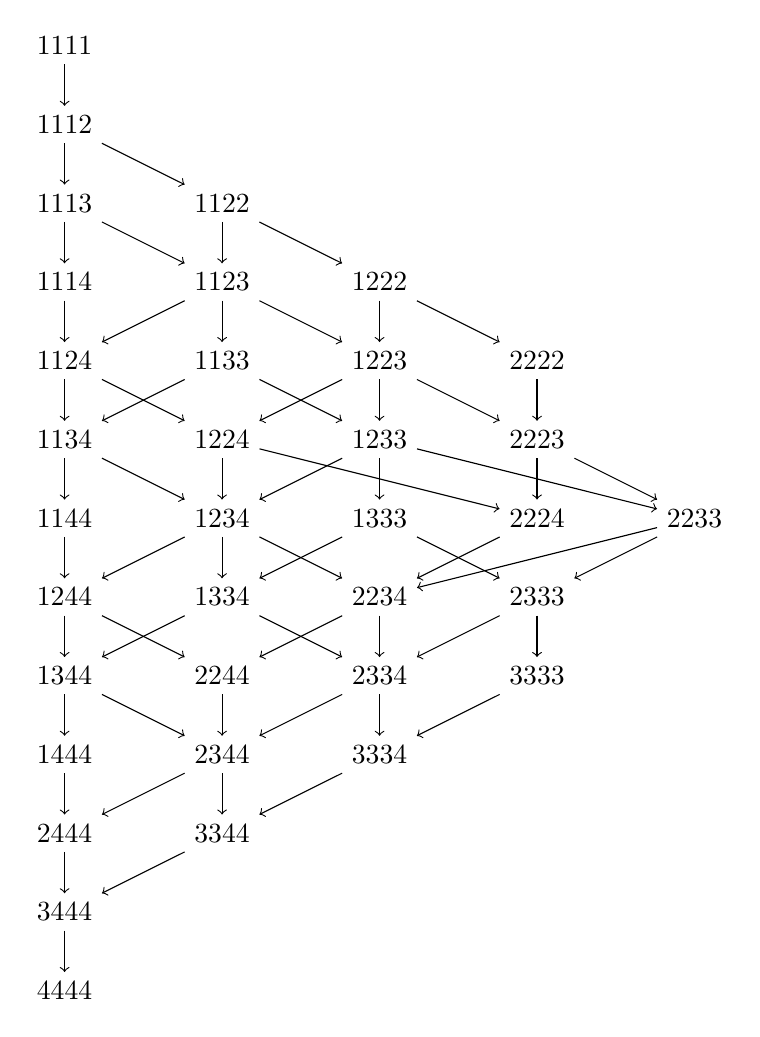
\begin{tikzpicture}
%Nodes
\node  (node1111) at (0,12) {1111};

\node  (node1112) at (0,11) {1112};

\node  (node1113) at (0,10) {1113};
\node  (node1122) at (2,10) {1122};

\node  (node1114) at (0,9) {1114};
\node  (node1123) at (2,9) {1123};
\node  (node1222) at (4,9) {1222};

\node  (node1124) at (0,8) {1124};
\node  (node1133) at (2,8) {1133};
\node  (node1223) at (4,8) {1223};
\node  (node2222) at (6,8) {2222};

\node  (node1134) at (0,7) {1134};
\node  (node1224) at (2,7) {1224};
\node  (node1233) at (4,7) {1233};
\node  (node2223) at (6,7) {2223};

\node  (node1144) at (0,6) {1144};
\node  (node1234) at (2,6) {1234};
\node  (node1333) at (4,6) {1333};
\node  (node2224) at (6,6) {2224};
\node  (node2233) at (8,6) {2233};

\node  (node1244) at (0,5) {1244};
\node  (node1334) at (2,5) {1334};
\node  (node2234) at (4,5) {2234};
\node  (node2333) at (6,5) {2333};

\node  (node1344) at (0,4) {1344};
\node  (node2244) at (2,4) {2244};
\node  (node2334) at (4,4) {2334};
\node  (node3333) at (6,4) {3333};

\node  (node1444) at (0,3) {1444};
\node  (node2344) at (2,3) {2344};
\node  (node3334) at (4,3) {3334};

\node  (node2444) at (0,2) {2444};
\node  (node3344) at (2,2) {3344};

\node  (node3444) at (0,1) {3444};

\node  (node4444) at (0,0) {4444};

%Lines
\draw[->] (node1111) edge node[thick, auto] {} (node1112);

\draw[->] (node1112) edge node[thick, auto] {} (node1113);
\draw[->] (node1112) edge node[thick, auto] {} (node1122);

\draw[->] (node1113) edge node[thick, auto] {} (node1114);
\draw[->] (node1113) edge node[thick, auto] {} (node1123);

\draw[->] (node1114) edge node[thick, auto] {} (node1124);

\draw[->] (node1122) edge node[thick, auto] {} (node1123);
\draw[->] (node1122) edge node[thick, auto] {} (node1222);

\draw[->] (node1123) edge node[thick, auto] {} (node1223);
\draw[->] (node1123) edge node[thick, auto] {} (node1124);
\draw[->] (node1123) edge node[thick, auto] {} (node1133);

\draw[->] (node1124) edge node[thick, auto] {} (node1224);
\draw[->] (node1124) edge node[thick, auto] {} (node1134);

\draw[->] (node1133) edge node[thick, auto] {} (node1233);
\draw[->] (node1133) edge node[thick, auto] {} (node1134);

\draw[->] (node1134) edge node[thick, auto] {} (node1234);
\draw[->] (node1134) edge node[thick, auto] {} (node1144);

\draw[->] (node1144) edge node[thick, auto] {} (node1244);

\draw[->] (node1244) edge node[thick, auto] {} (node1344);
\draw[->] (node1244) edge node[thick, auto] {} (node2244);

\draw[->] (node1344) edge node[thick, auto] {} (node1444);
\draw[->] (node1344) edge node[thick, auto] {} (node2344);

\draw[->] (node1444) edge node[thick, auto] {} (node2444);

\draw[->] (node2444) edge node[thick, auto] {} (node3444);

\draw[->] (node3444) edge node[thick, auto] {} (node4444);


\draw[->] (node1222) edge node[thick, auto] {} (node1223);
\draw[->] (node1222) edge node[thick, auto] {} (node2222);

\draw[->] (node1223) edge node[thick, auto] {} (node1233);
\draw[->] (node1223) edge node[thick, auto] {} (node1224);
\draw[->] (node1223) edge node[thick, auto] {} (node2223);

\draw[->] (node1224) edge node[thick, auto] {} (node1234);
\draw[->] (node1224) edge node[thick, auto] {} (node2224);

\draw[->] (node1234) edge node[thick, auto] {} (node1244);
\draw[->] (node1234) edge node[thick, auto] {} (node1334);
\draw[->] (node1234) edge node[thick, auto] {} (node2234);

\draw[->] (node1334) edge node[thick, auto] {} (node1344);
\draw[->] (node1334) edge node[thick, auto] {} (node2334);

\draw[->] (node1233) edge node[thick, auto] {} (node1333);
\draw[->] (node1233) edge node[thick, auto] {} (node1234);
\draw[->] (node1233) edge node[thick, auto] {} (node2233);

\draw[->] (node1333) edge node[thick, auto] {} (node2333);
\draw[->] (node1333) edge node[thick, auto] {} (node1334);

\draw[->] (node2222) edge node[thick, auto] {} (node2223);

\draw[->] (node2223) edge node[thick, auto] {} (node2224);
\draw[->] (node2223) edge node[thick, auto] {} (node2233);

\draw[->] (node2224) edge node[thick, auto] {} (node2234);

\draw[->] (node2233) edge node[thick, auto] {} (node2234);
\draw[->] (node2233) edge node[thick, auto] {} (node2333);

\draw[->] (node2234) edge node[thick, auto] {} (node2334);
\draw[->] (node2234) edge node[thick, auto] {} (node2244);

\draw[->] (node2334) edge node[thick, auto] {} (node2344);
\draw[->] (node2334) edge node[thick, auto] {} (node3334);

\draw[->] (node2244) edge node[thick, auto] {} (node2344);

\draw[->] (node2344) edge node[thick, auto] {} (node2444);
\draw[->] (node2344) edge node[thick, auto] {} (node3344);

\draw[->] (node3344) edge node[thick, auto] {} (node3444);

\draw[->] (node2333) edge node[thick, auto] {} (node3333);
\draw[->] (node2333) edge node[thick, auto] {} (node2334);

\draw[->] (node3333) edge node[thick, auto] {} (node3334);

\draw[->] (node3334) edge node[thick, auto] {} (node3344);
\end{tikzpicture}
\end{center}
\end{minipage}




\end{document}
